\documentclass[12pt]{article}
\usepackage[T1]{fontenc}
\usepackage[polish]{babel}
\usepackage[utf8]{inputenc}
\newcommand{\BibTeX}{{\sc Bib}\TeX} 
\usepackage{graphicx}
\usepackage{amsfonts}
\usepackage[hidelinks]{hyperref}
\usepackage{float}

\usepackage{xcolor}
\usepackage{listings}
\lstset{
	basicstyle=\ttfamily\small,
	keywordstyle=\color{blue},
	commentstyle=\color{gray},
	stringstyle=\color{green!50!black},
	backgroundcolor=\color{black!5},
	showstringspaces=false,
	breaklines=true,
	frame=single,
	columns=flexible,
	keepspaces=true
}

\setlength{\textheight}{21cm}

\title{{\bf Zadanie nr 1 - Generacja sygnału i szumu}\linebreak
Cyfrowe Przetwarzanie Sygnałów}
\author{Bartosz Kołaciński, 251554 \and Jakub Rosiak, 251620}
\date{\today}

\begin{document}
\clearpage\maketitle
\thispagestyle{empty}
\newpage
\setcounter{page}{1}
\section{Cel zadania}

Celem zadania jest utworzenie programu umożliwiającego generację sygnałów i szumów o określonych parametrach, umożliwienie wykonywania na nich podstawowych operacji (dodawanie, odejmowanie, mnożenie i dzielenie) oraz ich graficzną prezentacje. Dodatkowo program umożliwia zapis i odczyt utworzonych sygnałów do plików binarnych. 

\section{Instrukcja korzystania z aplikacji}

\subsection{Instalacja aplikacji}

Wymagania:
\begin{itemize}
	\item git
	\item Python 3.13+
\end{itemize}

\begin{lstlisting}[language=bash]
  # Pobranie kodu i przejscie do folderu projektu
  git clone https://github.com/bkolacinski/cyfrowe-przetwarzanie-sygnalow.git
  cd cyfrowe-przetwarzanie-sygnalow
	
  # Utworzenie wirtualnego srodowiska
  python -m venv .venv
	
  # Aktywacja wirtualnego srodowiska 
  .\.venv\Scripts\activate  # Windows
  source .venv/Scripts/activate  # Linux / MacOS
	
  # Pobranie zaleznosci
  pip install -r requirements.txt
	
  # Uruchomienie programu
  streamlit run src/streamlit_app.py
\end{lstlisting}

\noindent
Po wykonaniu instalacji kodu oraz zależności, aby ponownie uruchomić program konieczne jest tylko wykonanie ostatniego polecenia (dodatkowo aktywacja wirtualnego środowiska, jeśli )

\newpage
\subsection{Korzystanie z aplikacji}

Po wykonaniu ostatniego polecenia w przeglądarce powinno pojawić się nowa karta z aplikacją. Jeżeli tak się nie stanie należy wejść na \href{http://localhost:8501}{\texttt{localhost:8501}}.

\begin{figure}[H]
	\centering
	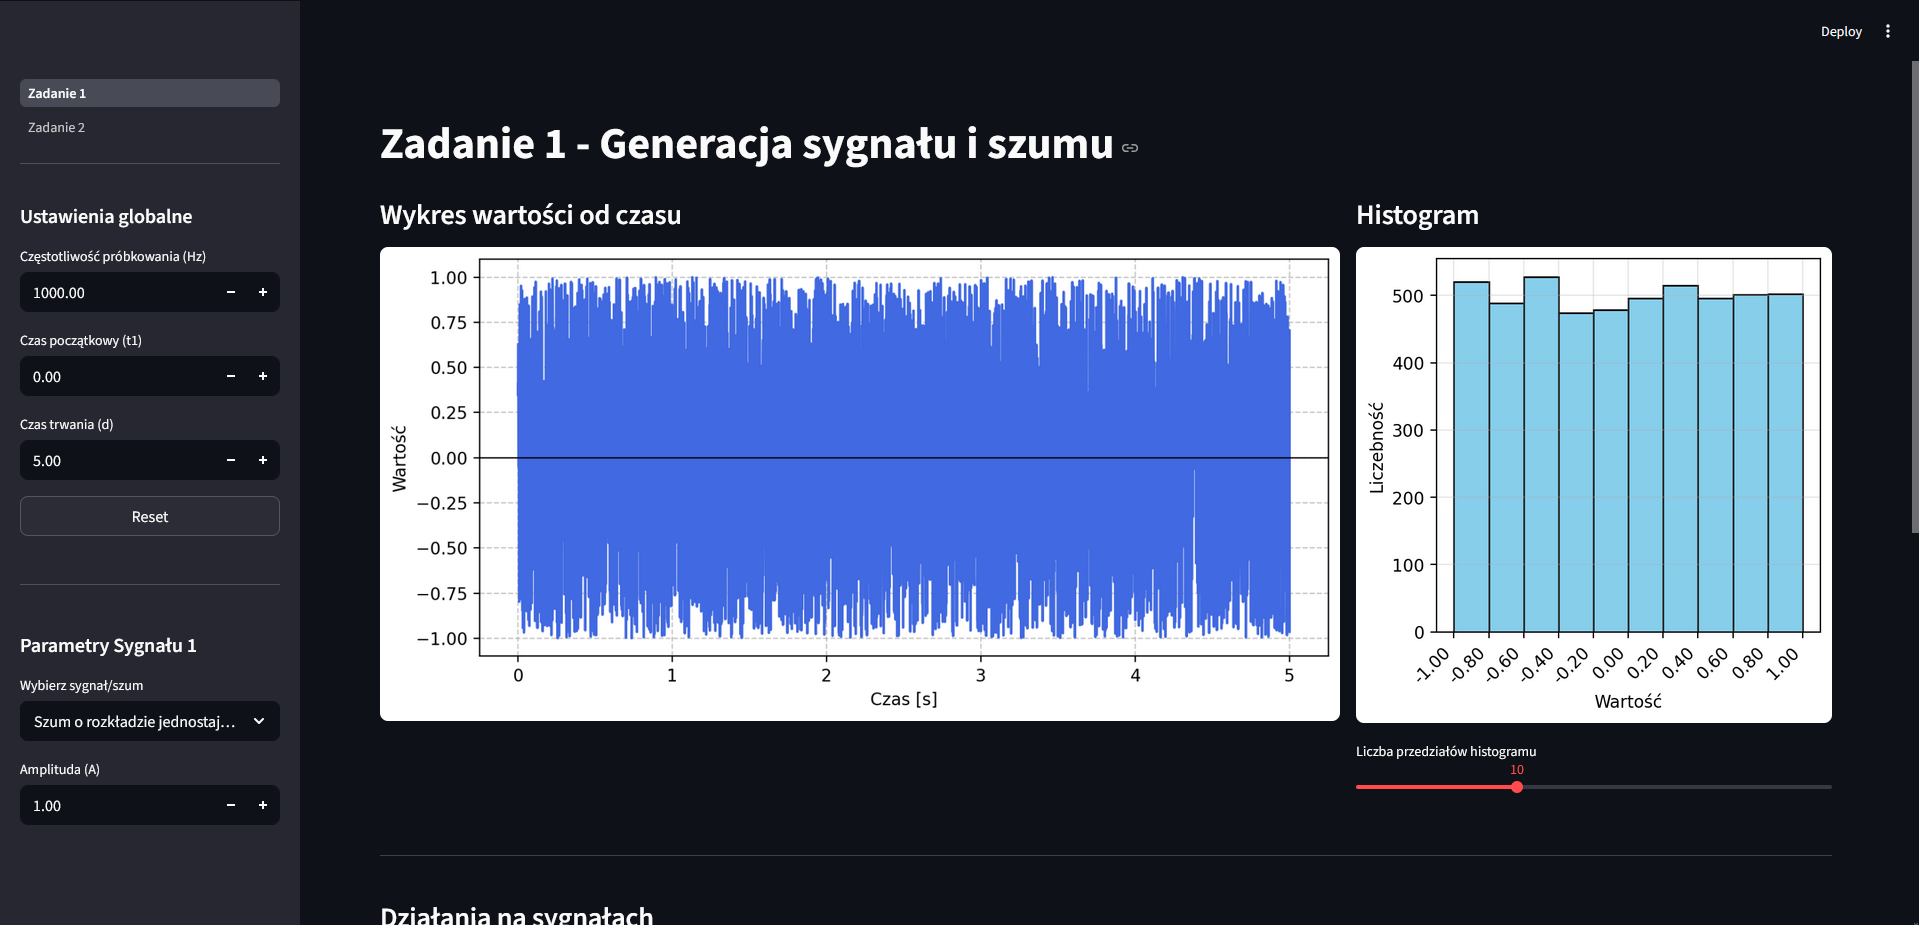
\includegraphics[width=\linewidth]{img/zad_1_1}
	\caption{Wygląd aplikacji w przeglądarce}
	\label{fig:zad11}
\end{figure}

\begin{figure}[H]
	\centering
	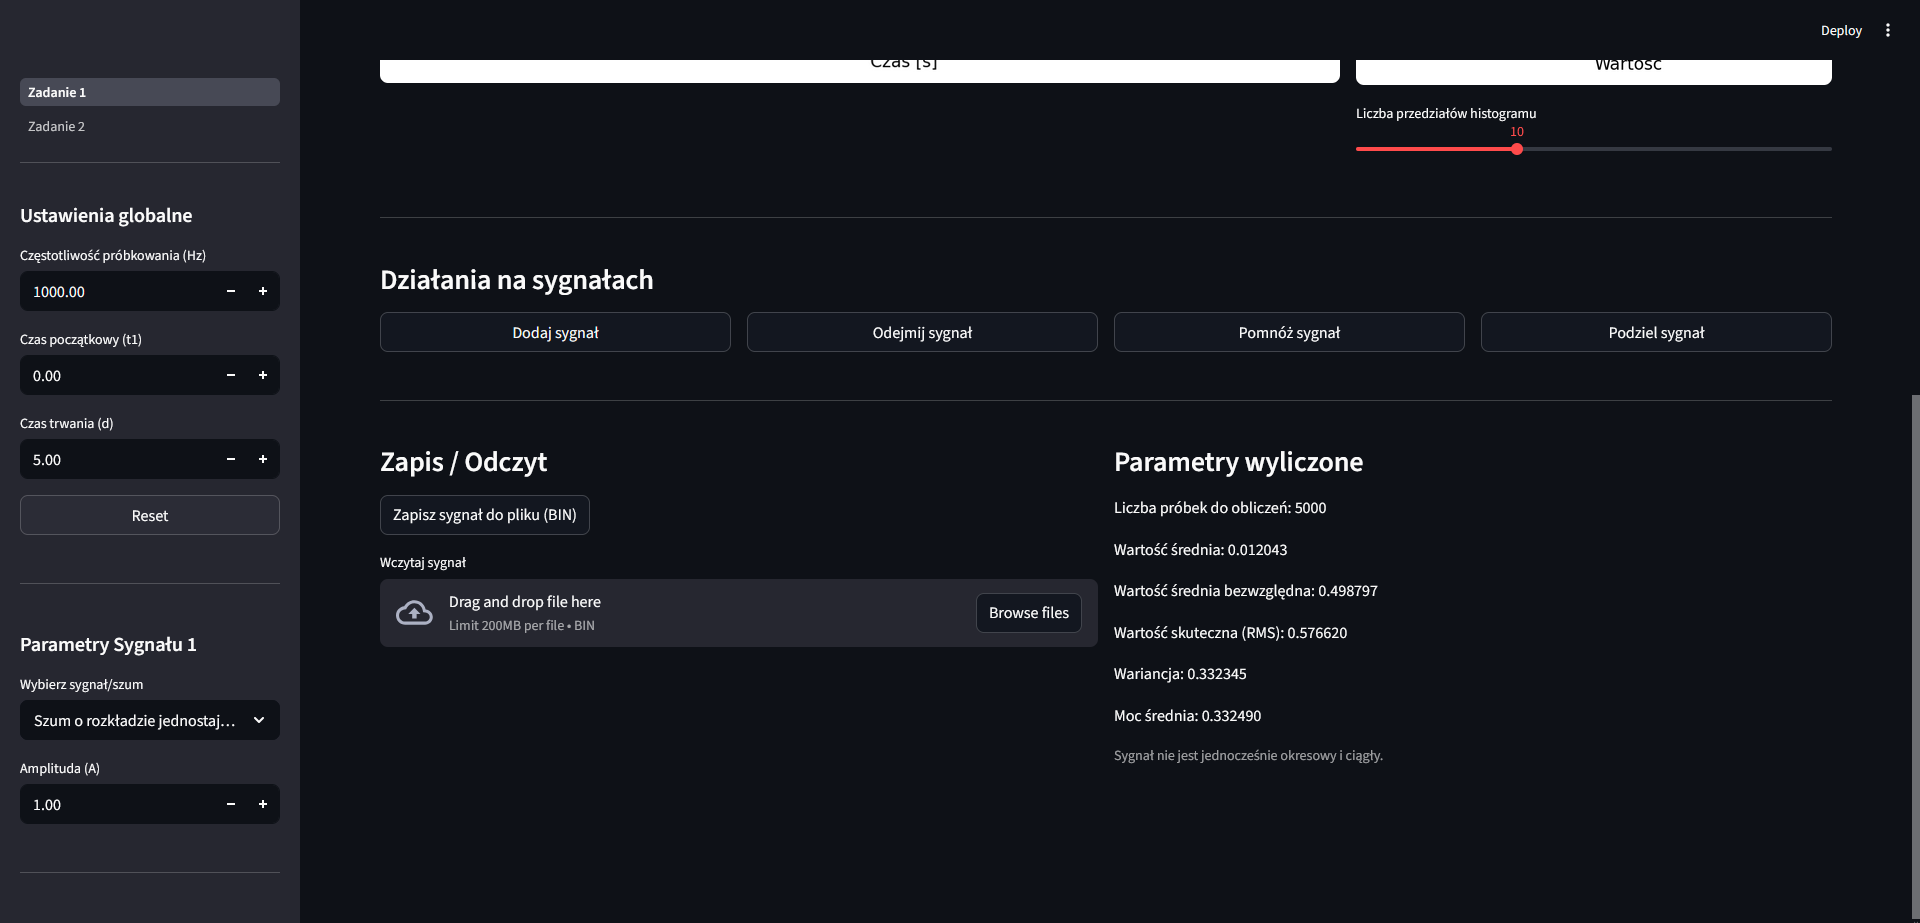
\includegraphics[width=\linewidth]{img/zad_1_2}
	\caption{Dalsza część aplikacji (po przewinięciu strony)}
	\label{fig:zad12}
\end{figure}

\newpage
\noindent
\textbf{Panel po lewej stronie umożliwia:}
\begin{itemize}
	\item \textbf{Konfiguracja parametrów globalnych} – definiowanie ustawień wspólnych dla wszystkich przetwarzanych sygnałów.
	\item \textbf{Przywracanie ustawień} – przycisk „Reset” pozwala na szybki powrót do wartości domyślnych wszystkich parametrów.
	\item \textbf{Zarządzanie sygnałami} – wybór typu sygnału oraz szczegółowa konfiguracja jego parametrów.
\end{itemize}

\noindent
\textbf{Główna część strony umożliwia:}
\begin{itemize}
	\item \textbf{Wizualizację danych} – generowanie wykresu czasowego funkcji oraz odpowiadającego jej histogramu (z możliwością regulacji liczby przedziałów/słupków za pomocą suwaka).
	\item \textbf{Operacje na sygnałach} – dodawanie nowych składowych (domyślnie sygnał S1). W przypadku dużej liczby sygnałów panel boczny automatycznie udostępnia funkcję przewijania (scrollowania).
	\item \textbf{Archiwizację} – zapis bieżącej konfiguracji sygnału do pliku oraz odczyt wcześniej zapisanych danych.
	\item \textbf{Analizę parametrów} – bieżący podgląd wartości statystycznych i parametrów wyliczonych dla aktualnie wyświetlanego sygnału.	
\end{itemize}

\section{Metody generowania danych}

Do generowania punktów wykorzystywana jest funkcja \texttt{get\_time\_vector()}, która tworzy równomiernie rozłożone próbki w przedziale czasu od chwili początkowej \(t_1\) do chwili końcowej \(t_1 + d\), gdzie \(d\) to czas trwania sygnału. Liczba próbek zależy od częstotliwości próbkowania \(f_s\).
\begin{lstlisting}[language=python]
def get_time_vector(t1, d, fs):
	num_samples = int(d * fs)
	t = np.linspace(t1, t1 + d, num_samples, endpoint=True)
	return t
\end{lstlisting}

\noindent
Funkcje \cite{cps-zadanie1-instrukcja}


\section{Opis implementacji}

Aplikacja została zaimplementowana w języku Python, z wykorzystaniem kilku kluczowych bibliotek wspierających zarówno logikę obliczeniową, jak i warstwę wizualną.

Do budowy interfejsu użytkownika wykorzystano bibliotekę Streamlit, która umożliwia szybkie tworzenie interaktywnych aplikacji webowych. Generowanie wykresów realizowane jest przy użyciu biblioteki Matplotlib, natomiast operacje numeryczne i przetwarzanie danych wykonywane są z pomocą NumPy. Do zapisu i odczytu danych z plików zastosowano bibliotekę msgpack, zapewniającą wydajną serializację danych.

W trakcie implementacji skupiono się na modularności kodu oraz czytelnym podziale odpowiedzialności pomiędzy poszczególne pliki.

\subsection*{Struktura projektu}

\begin{itemize}
	\item \texttt{streamlit\_app.py} -- główny plik aplikacji, odpowiedzialny za konfigurację i uruchomienie interfejsu Streamlit
	\item \texttt{signal\_io.py} -- moduł obsługujący zapis i odczyt danych sygnałów z plików
	\item \texttt{functions.py} -- zbiór funkcji generujących sygnały wykorzystywane w aplikacji
	\item \texttt{pages/zadanie1.py} -- implementacja strony odpowiadającej zadaniu 1 w aplikacji
\end{itemize}

\noindent
Funkcje wykorzystane w niniejszym sprawozdaniu zostały zaczerpnięte z instrukcji \cite{cps-zadanie1-instrukcja}. Niektóre wzory zostały uproszczone w celu czytelniejszej prezentacji, na przykład poprzez podstawienie wartości średniej i odchylenia standardowego w wzorze na szum gaussowski oraz jego skrócenie.

\newpage
\section{Eksperymenty}

\subsection{Eksperyment 1}
Analizowano sygnał będący sumą sygnału sinusoidalnego o amplitudzie 1.0 i okresie 1.2 oraz sygnału prostokątnego o amplitudzie 1.0 i okresie 1.0. Celem było zaobserwowanie wpływu dodania sygnału prostokątnego na przebieg wynikowy.

\begin{figure}[H]
    \centering
    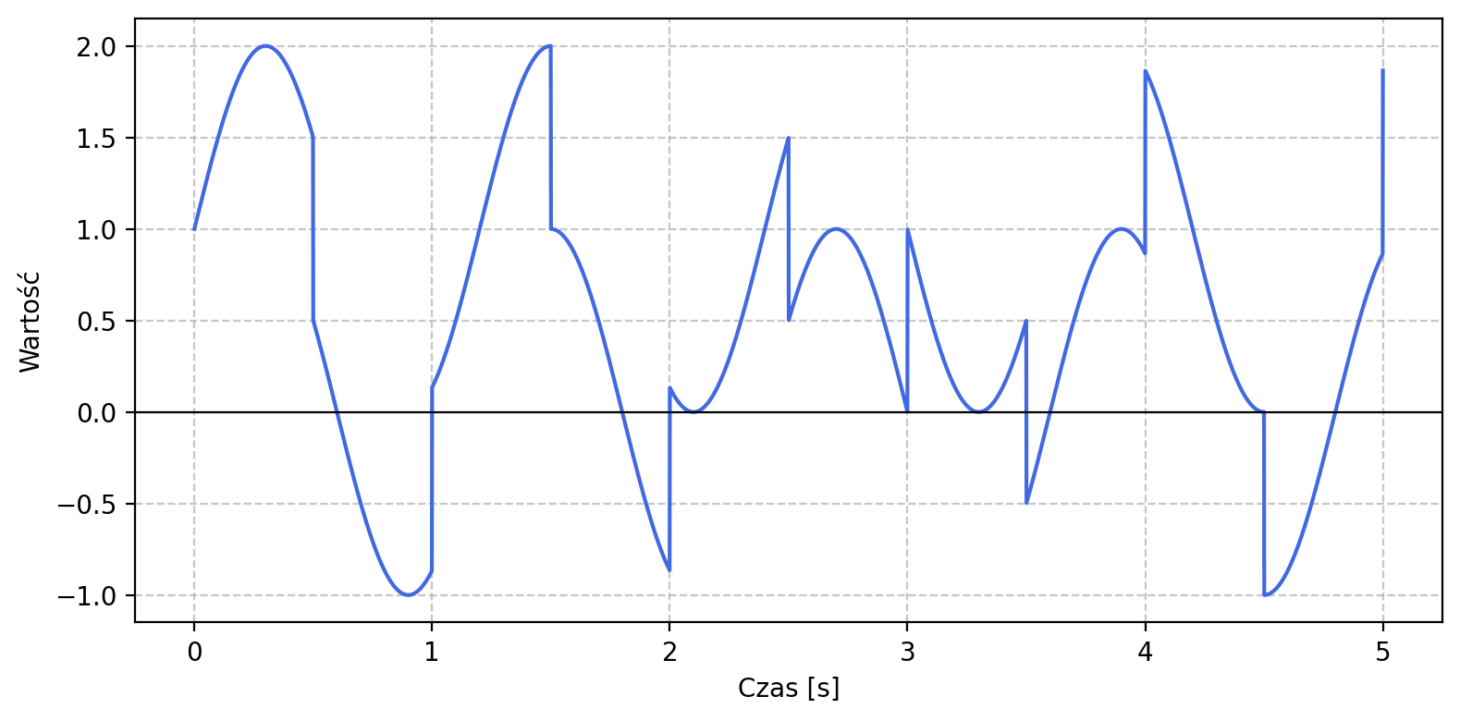
\includegraphics[width=0.8\textwidth]{img/eksperyment_1_1.png}
    \caption{Przebieg sygnału wynikowego}
\end{figure}

\begin{figure}[H]
    \centering
    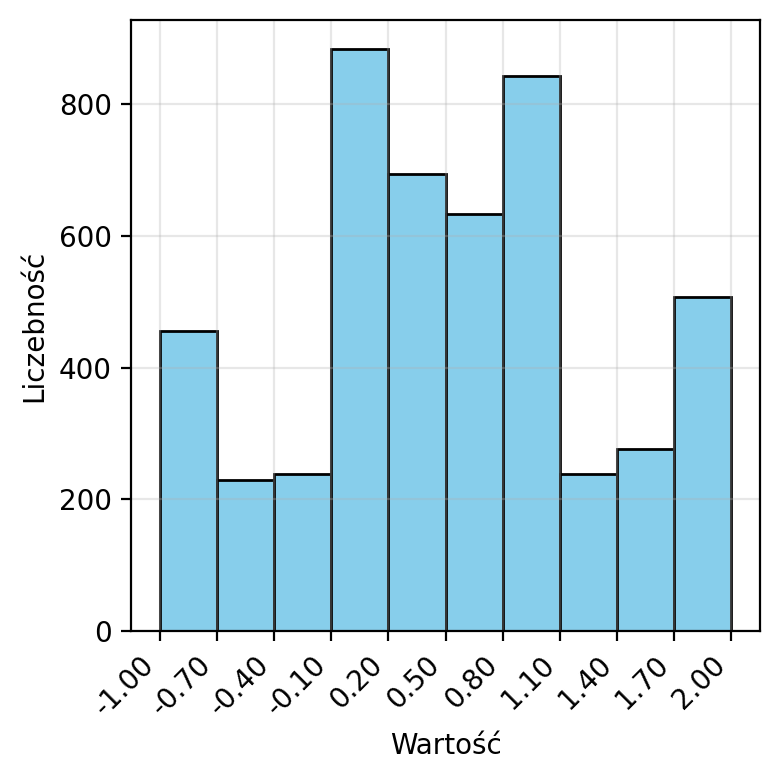
\includegraphics[width=0.6\textwidth]{img/eksperyment_1_1_histogram.png}
    \caption{Histogram wartości sygnału}
\end{figure}

\subsection{Eksperyment 2}
Analizowano sygnał sinusoidalny o amplitudzie 1.0 i okresie 1.8, od którego odjęto szum gaussowski o amplitudzie 1.5. Celem było zbadanie wpływu szumu na kształt sygnału oraz jego rozkład wartości.

\begin{figure}[H]
    \centering
    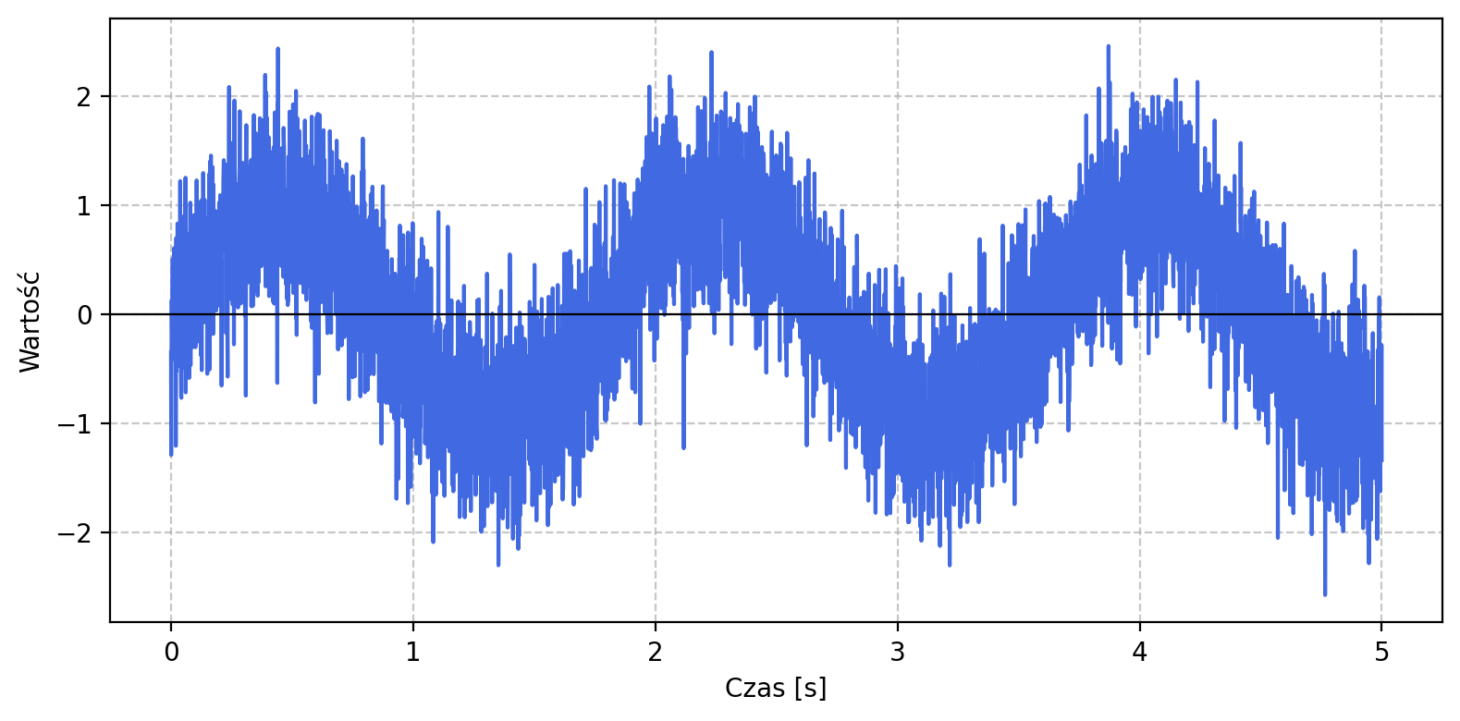
\includegraphics[width=0.8\textwidth]{img/eksperyment_1_2.png}
    \caption{Przebieg sygnału z szumem}
\end{figure}

\begin{figure}[H]
    \centering
    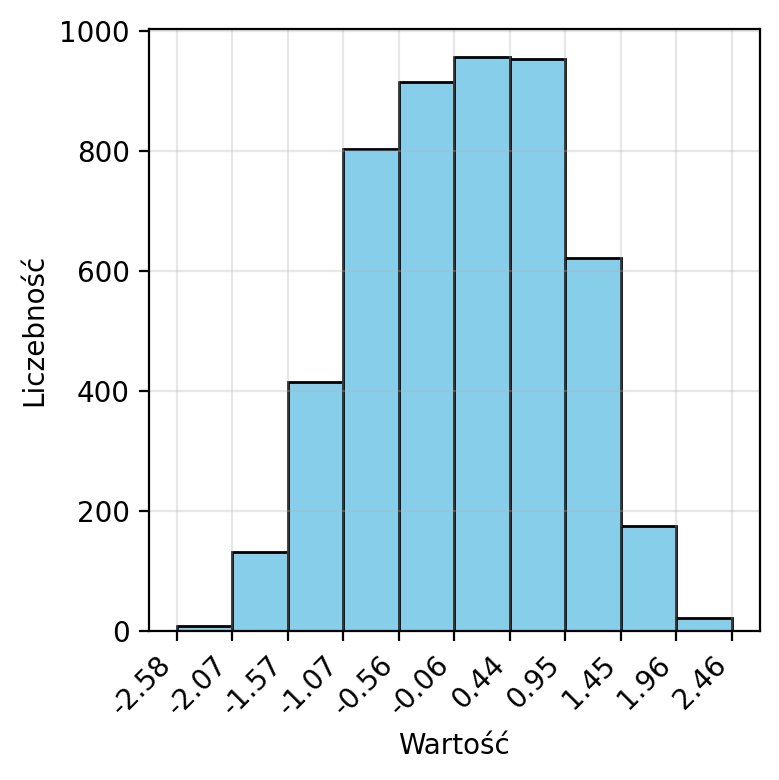
\includegraphics[width=0.6\textwidth]{img/eksperyment_1_2_histogram.png}
    \caption{Histogram wartości sygnału}
\end{figure}

\subsection{Eksperyment 3}
Analizowano sygnał powstały jako iloczyn sygnału sinusoidalnego o amplitudzie 1.0 i okresie 2.0 oraz sygnału trójkątnego o amplitudzie 0.8 i okresie 1.5, z dodanym szumem gaussowskim o amplitudzie 0.5. Celem było zbadanie wpływu modulacji oraz szumu na przebieg i rozkład wartości sygnału.

\begin{figure}[H]
    \centering
    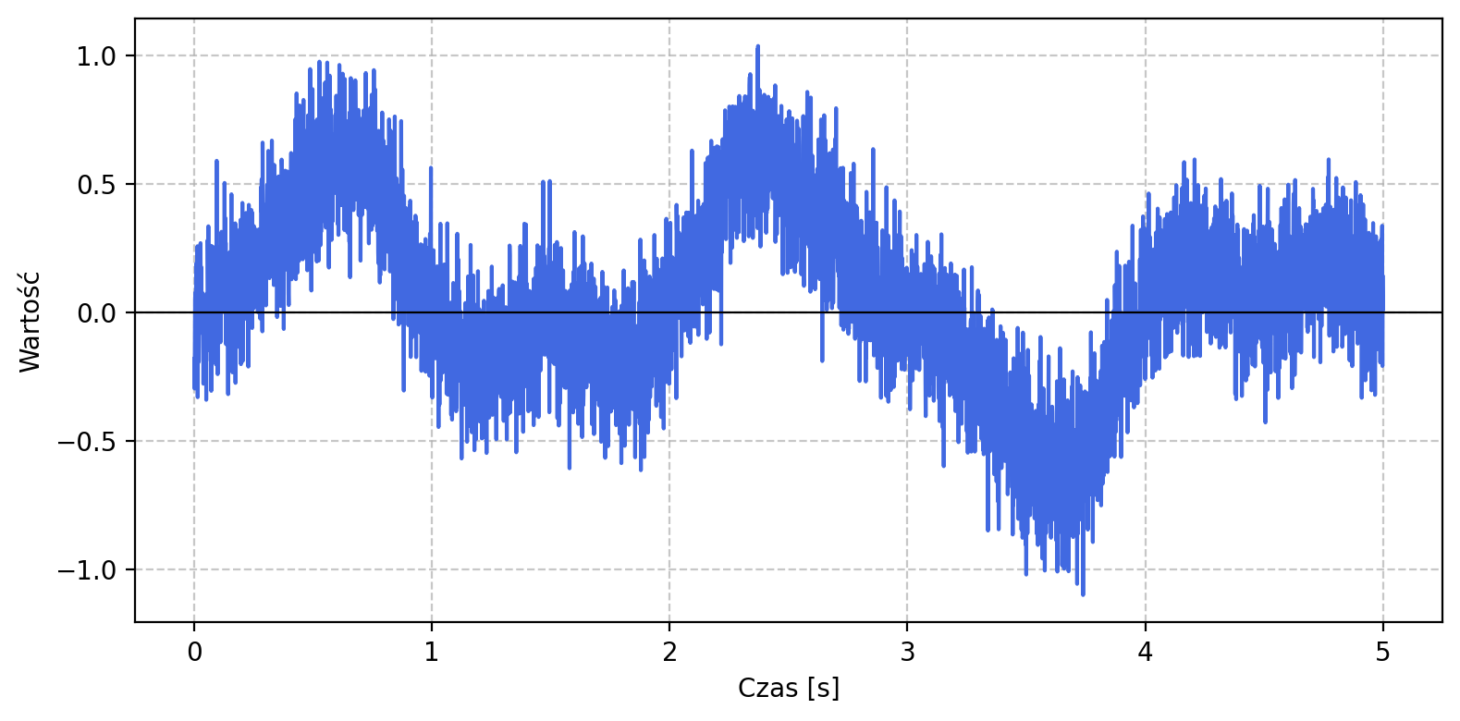
\includegraphics[width=0.8\textwidth]{img/eksperyment_1_3.png}
    \caption{Przebieg sygnału wynikowego}
\end{figure}

\begin{figure}[H]
    \centering
    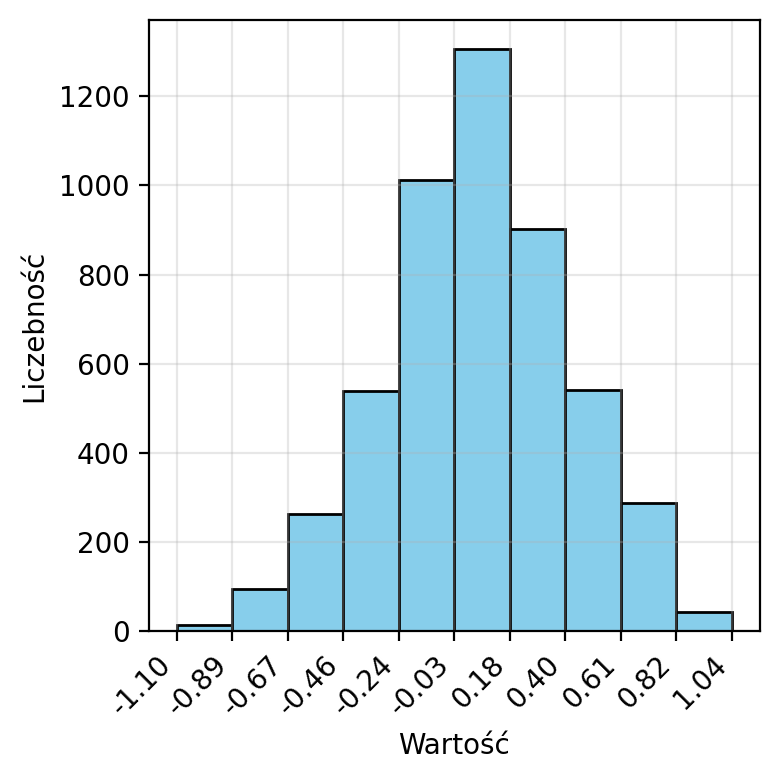
\includegraphics[width=0.6\textwidth]{img/eksperyment_1_3_histogram.png}
    \caption{Histogram wartości sygnału}
\end{figure}

\newpage
\section{Wnioski}

Zrealizowana aplikacja umożliwia intuicyjną generację oraz analizę sygnałów i szumów o zadanych parametrach. Zastosowanie interfejsu Streamlit znacząco upraszcza interakcję z użytkownikiem i pozwala na szybkie testowanie różnych konfiguracji.

Zaobserwowano, że zmiana parametrów takich jak częstotliwość próbkowania czy czas trwania sygnału ma bezpośredni wpływ na dokładność odwzorowania przebiegu. Z kolei dodanie szumu powoduje wyraźne zmiany w rozkładzie wartości, co jest widoczne na histogramach.

Implementacja podstawowych operacji arytmetycznych na sygnałach pozwala na łatwe badanie ich wzajemnych zależności. Dodatkowo możliwość zapisu i odczytu danych zwiększa funkcjonalność aplikacji i umożliwia powrót do wcześniej analizowanych przypadków.

Modularna struktura projektu ułatwia jego rozwój oraz utrzymanie.

\renewcommand\refname{Bibliografia}
\bibliographystyle{plain}
\bibliography{bibliografia}

\end{document}
